\documentclass[journal, a4paper]{IEEEtran}
\usepackage{graphicx}
\usepackage{url} 
\usepackage{amsmath}
\begin{document}

% Define document title and author
	\title{Homework 1: N-gram Language Models}
	\author{Guangyu Lin, EID: gl8429
}
	\markboth{CS 388 Natural Language Processing - University of Texas at Austin}{}
	\maketitle

% Write abstract here
\begin{abstract}
	The short report is intended to present homework 1, N-gram Language Models. We modified a simple, typical N-gram language model into backward bigram model and bidirectional bigram model. Then we trained and experimentally tested them on English datasets, Airline Booking Conversations(ATIS), Wall Street Journal(WSJ), and Brown. Finally, we present tables and figures of comparative results, then we concludes backward bigram model is a little better than forward bigram model in diverse dataset and forward bigram model is better in spoken discourse. And bidirectional bigram model is the best one of three, because it is a combinational prediction of another two models.
\end{abstract}

% Each section begins with a \section{title} command
\section{Introduction}
	% \PARstart{}{} creates a tall first letter for this first paragraph
	This report explores a modification of a simple, typical N-gram language model~\cite{MJH06} and experimentally test it on English dataset, which includes Airline Booking Conversations(ATIS), Wall Street Journal(WSJ), and Brown. The first modification is to produce a "backward" bigram model that models the generation of a sentence from right to left. The second modification is to combine the forward and backward model. Additionally, we weight the prediction of both models equally when interpolating a probability for each word/token in the sentence. For each bigram language model, we produce a trace analogous to the sample BigramModel trace file. Then, we draw several tables and several figures of comparative results and states a discussion about the difference and similarities which we found.~\cite{HOP96}
	
	The report is organized as following, the algorithms of backward bigram model and bidirectional bigram model are described briefly in Section~\ref{algorithm}. The results table and figure is provided in Section~\ref{result}. We discuss our results in Section~\ref{discuss}. And Section~\ref{conclude} is the conclusion of the report.

% Main Part
\section{Algorithms}\label{algorithm}
\vspace{3mm}
\subsection{Backward Bigram Model}
The one significant difference between a left-to-right and a right-to-left(backward) model is that the backward model's final prediction is to predict sentence-start($<S>$) rather than sentence-end($</S>$). Therefore, I modify the original code of Bigram Model before I train data and calculate the sentence probabilities by reversing the sentences. For smoothing part, we use the same weights as in forward bigram model, $\frac{1}{10}$ on the unigram and $\frac{9}{10}$ on the bigram and we also replace the leftmost token of each type with "$<UNK>$" token. Then we derived from the following formula:
\[
  \frac{1}{10}p_{unigram} + \frac{9}{10}p_{backward-bigram}
\]

%\vspace{3mm}

\subsection{Bidirectional Bigram Model}
Bidirectional Bigram Model combines the forward and backward model. When determining the probability of a word in the sentence, it should use both the estimate from its forward and backward contexts by linearly interpolating the probability predicted for that token by BigramMode and BackwardBigramModel. By default, just weight the prediction of both modes equally when interpolating a probability for each word/token in the sentence.~\cite{HOP96}

To calculate the combination probability of these to models, I derived from the following formula:

\[
  \frac{1}{10}p_{unigram} + \frac{9}{10}\left(\frac{1}{2}p_{forward-bigram} + \frac{1}{2}p_{backward-bigram}\right)
\]
We can also play with different ratio of weight of the prediction.

\section{Experiment Results}\label{result}

We train and test three datasets (ATIS, WSJ, BROWN) with a ratio of 9:1. Table~\ref{tab:1} is the results of training dataset: ATIS and Table~\ref{tab:2} is the results of testing dataset: ATIS. The results include preplexity and word preplexity. Similarly,  Table~\ref{tab:3} - Table~\ref{tab:6} are training and testing results of the other two datasets.

	\begin{table}[!hbt]
		\begin{center}
		% Title of the table
		\caption{Training Data: atis}
		\label{tab:1}
		\begin{tabular}{|c|c|c|}
			\hline
			Model & Preplexity & Word Preplexity\\
			\hline
			 Forward Bigram & 9.043  & 11.636 \\ \hline
			 Backward Bigram & 9.013 &  10.592 \\ \hline
			Bidirectional Bigram & 6.079 & 7.235 \\
			\hline
		\end{tabular}
		\end{center}
	\end{table}
\vspace{-7mm}	
	\begin{table}[!hbt]
		\begin{center}
		% Title of the table
		\caption{Testing Data: atis}
		\label{tab:2}
		\begin{tabular}{|c|c|c|}
			\hline
			Model & Preplexity & Word Preplexity\\
			\hline
			 Forward Bigram &19.341  & 24.054 \\ \hline
			 Backward Bigram & 19.364 &  27.161 \\ \hline
			Bidirectional Bigram & 10.227 & 12.700 \\
			\hline
		\end{tabular}
		\end{center}
	\end{table}
	
\vspace{-7mm}	
	\begin{table}[!hbt]
		\begin{center}
		% Title of the table
		\caption{Training Data: WSJ}
		\label{tab:3}
		\begin{tabular}{|c|c|c|}
			\hline
			Model & Preplexity & Word Preplexity\\
			\hline
			 Forward Bigram &74.268  & 88.890 \\ \hline
			 Backward Bigram  & 74.268 &  86.660 \\ \hline
			Bidirectional Bigram & 40.204 & 46.514 \\
			\hline
		\end{tabular}
		\end{center}
	\end{table}
\vspace{-7mm}	
	\begin{table}[!hbt]
		\begin{center}
		% Title of the table
		\caption{Testing Data: WSJ}
		\label{tab:4}
		\begin{tabular}{|c|c|c|}
			\hline
			Model & Preplexity & Word Preplexity\\
			\hline
			 Forward Bigram &219.715  & 275.118 \\ \hline
			 Backward Bigram  & 219.520 &  266.352 \\ \hline
			Bidirectional Bigram & 104.796 & 126.113 \\
			\hline
		\end{tabular}
		\end{center}
	\end{table}

	\begin{table}[!hbt]
		\begin{center}
		% Title of the table
		\caption{Training Data: BROWN}
		\label{tab:5}
		\begin{tabular}{|c|c|c|}
			\hline
			Model & Preplexity & Word Preplexity\\
			\hline
			 Forward Bigram & 93.519  & 113.360 \\ \hline
			 Backward Bigram  & 93.509 &  110.783 \\ \hline
			Bidirectional Bigram & 52.375 & 61.469 \\
			\hline
		\end{tabular}
		\end{center}
	\end{table}

	\begin{table}[!hbt]
		\begin{center}
		% Title of the table
		\caption{Testing Data: BROWN}
		\label{tab:6}
		\begin{tabular}{|c|c|c|}
			\hline
			Model & Preplexity & Word Preplexity\\
			\hline
			 Forward Bigram & 231.302  & 310.667 \\ \hline
			 Backward Bigram  & 231.206 &  299.686 \\ \hline
			Bidirectional Bigram & 130.157 & 167.487 \\
			\hline
		\end{tabular}
		\end{center}
	\end{table}


\section{Discussion}\label{discuss}
\subsection{Forward V.S. Backward Bigram Models}
As far as we know, forward bigram models is to predict where the sentences end, whereas, backward bigram models is to predict where the sentences begin.

From the previous six tables, we find that the preplexity or word preplexity of the training data of each dataset is better than of the testing data of each dataset, which is obvious. We also find that the preplexity of ATIS is better than the other two datasets because of its small. For ATIS(airline booking conversations), the forward bigram model is better than the backward bigram model, which may because of spoken discourse. At the beginning of a sentence, we would like to insert greetings or other interjections.

For other two datasets, WSJ(Wall Street Journal) and Brown, the backward bigram model is better than the forward bigram model, which may because of their diverse datasets.

\subsection{Bidirectional V.S. Backward V.S. Forward Bigram Models}
To deep dive the results tables, we combine some data from the previous tables, then we get Table~\ref{comp:1} and Table~\ref{comp:2}, which are directly in Figure~\ref{fig:tf_plot1} and Figure~\ref{fig:tf_plot2} . For each dataset, forward bigram model is similar to backward bigram model and bidirectional bigram model is almost twice better than the other two models. Why is that? In my opinion, the forward bigram models look like $<left, ?>$ and  the backward bigram models look like$ <?, right>$. The combinational bidirectional bigram models look like, $<left, ?>$ and $<?, right>$, which combine the predictions of forward and backward bigram models. Therefore, the word preplexity is better than the other two models.
	
	\begin{table}[!hbt]
		\begin{center}
		% Title of the table
		\caption{Word Preplexity of Training Data: ATIS, WSJ, BROWN}
		\label{comp:1}
		\begin{tabular}{|c|c|c|c|}
			\hline
			Dataset & Forward Bigram & Backward Bigram & Bidirectional Bigram\\
			\hline
			 ATIS & 10.591  & 11.636 & 7.235 \\ \hline
			 WSJ &  88.890 &  86.660 & 46.514 \\ \hline
			BROWN & 113.360 & 110.783 & 61.469 \\
			\hline
		\end{tabular}
		\end{center}
	\end{table}
	
		\begin{figure}[!hbt]
		\begin{center}
		\includegraphics[width=\columnwidth]{WofTrain}
		% Create a subtitle for the figure.
		\caption{Word Preplexity of Training Data}
		\label{fig:tf_plot1}
		\end{center}
	\end{figure}

	\begin{table}[!hbt]
		\begin{center}
		% Title of the table
		\caption{Word Preplexity of Testing Data: ATIS, WSJ, BROWN}
		\label{comp:2}
		\begin{tabular}{|c|c|c|c|}
			\hline
			Dataset & Forward Bigram & Backward Bigram & Bidirectional Bigram\\
			\hline
			 ATIS & 24.054  & 27.161 & 12.700 \\ \hline
			 WSJ &  275.118 &  266.352 & 126.113 \\ \hline
			BROWN & 310.667 & 299.686 & 167.487 \\
			\hline
		\end{tabular}
		\end{center}
	\end{table}

	\begin{figure}[!hbt]
		\begin{center}
		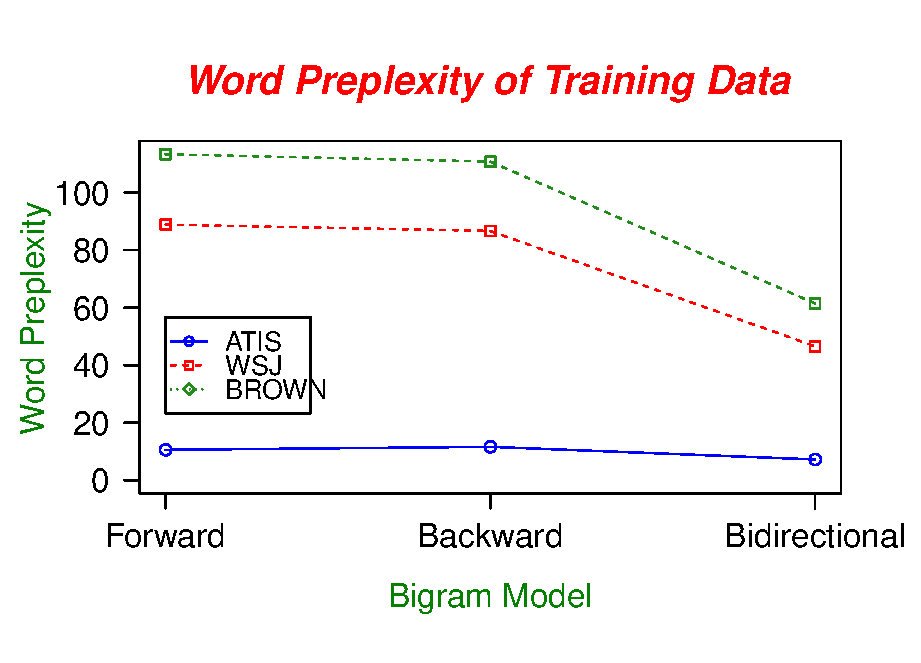
\includegraphics[width=\columnwidth]{WofTest}
		% Create a subtitle for the figure.
		\caption{Word Preplexity of Testing Data}
		\label{fig:tf_plot2}
		\end{center}
	\end{figure}

\section{Conclusion}\label{conclude}
	In this report, we talked about the algorithms of backward bigram models and bidirectional bigram models. From the experimental results, we find backward bigram model is a little better than forward bigram model in diverse dataset and forward bigram model is better in spoken discourse. And bidirectional bigram model is the best one of three, because it is a combinational prediction of another two models.
	
% Now we need a bibliography:
\begin{thebibliography}{5}

	%Each item starts with a \bibitem{reference} command and the details thereafter.
	\bibitem{HOP96} % Transaction paper
	https://www.cs.utexas.edu/~mooney/cs388/hw1.html

	\bibitem{MJH06} % Conference paper
	 Martin, James H., and Daniel Jurafsky. "Speech and language processing." International Edition (2000).


\end{thebibliography}

% Your document ends here!
\end{document}